
%\newcommand{\SHAW}{{\em {\sffamily BRIDGE}}}
 In their recent   2018 IEEE Software paper ``Bridging the Gap
From Research to Practical Advice'', 
Le~Goues, Shaw et al.~\cite{Goues18}
  lamented the poor connection between research discoveries and practitioner needs. To bridge that
 gap, they proposed  ``a system that allows researchers and
practitioners to reliably synthesize research results into actionable, real-world guidance,'' and literature reviews that make ``explicit recommendations on practice,
clearly labeled with strength of recommendation reflecting the level of rigor of the underlying evidence.''
There is a clear need for such a system: 
\bi
\item
On average, SE research   papers  earn less than one citation per paper~\cite{Mathew_2018}.
\item
This means that researchers and practitioners may miss important information.  
\item
Something needs to be done to stop so much research being not cited, forgotten, and hence wasted. 
\ei
Systematic Literature Reviews (SLRs) are one of the key approaches researchers use to systematically identify, analyze, and synthesize the research on a particular topic~\cite{Kitchenham:04,Kitchenham_Charters:07,Kitchenham-etal:04}.
The goal of an SLR is to provide a general overview of the current state of knowledge regarding topics or questions of interest.
Therefore, SLRs could be a key method to address the goals of 
Le  Goues,  Shaw  et  al.
Based on our own experience in the SLR and more general literature review space~\cite{Yu2018,Yu2019,Mathew_2018,mathewSoft18,Menzies89,hassler2014outcomes,%
carver2013identifying,%
hassler2016identification,%
carver13z,%
Kakar_Carver_2012,%
Carver-etal:13,%
Al-Zubidy-Carver:14},
we have a thorough understanding of many of the technical challenges proposed by Le  Goues,  Shaw  et  al.

One of the primary limitations of the current SLR approach is that it is a heavily manual and time consuming work requiring weeks to months of effort.
For example, 
a recent study reports taking over 400 hours to complete the ``selection process'' (which is only one of the parts required to complete  an SLR)~\cite{Hassler:14}. 
%This same study reports taking 4 man-hours to review the quality of results that took seconds of computer time using an automated technique.
Hence, while the concept of an SLR is quite applicable to the Le  Goues,  Shaw  et  al. challenge, in its current state it may {\em not} be suitable (since it is so slow).

\begin{table}
\caption{A sample of the manual and automatic {\em methods} available for exploring the SE literature.
The point of this proposal is to offer the infrastructure 
that lets  SE
community decide   how to make best use of these methods.
Note that this list is incomplete since researchers are
regularly proposing new approaches. Note also that while we present this list as a {\em linear} process (running from top to bottom), 
SLRs are usually a {\em cyclic process} where analysts make multiple iterations  across  these methods.}\label{tbl:overview}
\begin{center}
 {\small
  \begin{tabular}{p{1.5cm}|p{5.5cm}|p{8.3cm}}
    \rowcolor{gray}   & \textcolor{white}{Primarily manual methods} & \textcolor{white}{Automated AI-based text mining methods }  \\
    \hline
    1a. 
    \newline Define \newline research \newline question &   Read many papers (a very slow process)~\cite{kitchenham2004evidence,keele2007guidelines,marshall2013tools}. If there was a repository on prior questions we could explore them. &
    \bii
    \item {\em Dcluster:} Clustering documents with (e.g.) topic modeling~\cite{Mathew_2018};
    \item {\em Qcluster:} Cluster old queries to find common patterns in queries (and results);
    \item Find the gaps (clusters with low frequencies).
    \eii  \\\hline\rowcolor{blue!10}
    1b. \newline Identify  keywords& Extract keywords from research question topics and known related literature &
    \bii
    \item Extract candidate words from {\em Qclusters};
    \item Use feature selection (e.g. TF-IDF or RELIEF on support vectors);
    \item Auditing the keywords with synonym discovery (PCA~\cite{Wold1987Principal}, Word2Vec~\cite{mikolov2013efficient}). 
    \item Use of information extraction tools~\cite{Cruzes2007Automated}. 
    \eii \\
    \hline
    1c.\newline Create search string  & 
    \bii
    \item
    Use synonyms of keywords to identify terms for search string.
    \item
    Using subject matter experts (hard, they are hard to find).
    \item
    Use of gold standard to refine the search string~\cite{zhang2011empirical}.
    \eii &
    \bii
    \item Construct most informative search strings using  active learning~\cite{Yu2018,Yu2019};
    \item Using  SVMs, cull terms  explore those found most often
    far from hyperspace boundary;
    \item Apply Word2Vec~\cite{mikolov2013efficient} to extend query with keyword synonyms (as done in \cite{georgeLN}).
    \eii \\
    \hline\rowcolor{blue!10}
    2. \newline Search databases \cite{kitchenham2004evidence,keele2007guidelines}& \bii
    \item
    Snowballing~\cite{jalali2012systematic}.
    \item
    Use various permutations of search string in each database (sometimes requiring multiple searches per database) 
    \eii & AI
    not required for this task. However, with automatic tool supports, the time required for this task can be  greatly reduced. 
    \\
    \hline
    3. \newline Select \newline relevant papers&Current practice: a mostly manual process~\cite{kitchenham2004evidence,keele2007guidelines,hassler2016identification}&
    \bii
    \item Use active learning trained/updated on human review results to recommend what next to be reviewed~\cite{Yu2018,Yu2019}.
    \item Try initializing queries with results from {\em Qcluster}~\cite{Pan2010A}. 
    \item Explore using information other than title and abstracts, e.g. use full-text information or summary of text~\cite{summary1,summary2,summary3} 
    \eii\\
    \hline\rowcolor{blue!10}
    4. \newline Assess\newline quality  & Some checklists (number of subjects, type of studies, e.g bad smells)~\cite{kitchenham2004evidence,keele2007guidelines} & Not currently explored
    by AI tools~\cite{marshall2013tools}. This might be a matter of entity recognition~\cite{manning-EtAl:2014:P14-5} over checklist but really cannot be definitive at this time. %This is an area where we hope some share data and shared conventions on how to integrate tools would enable more experiment and more tools in the future. 
    \\    \hline
    5. \newline Extract data & Manual process: reading the the actual papers. E.g. run over a pdf and add mark ups over the text (so you can localize where you look)~\cite{kitchenham2004evidence,keele2007guidelines}.  & Topic modeling and visualization tools might help here~\cite{Felizardo2010An,Torres2012Automatic}\\
    \hline\rowcolor{blue!10}
    6. \newline Synthesis of results &  Manual work with help using  tools~\cite{kitchenham2004evidence,keele2007guidelines,marshall2013tools}. & Visualization might be able to help this process~\cite{Cruzes2007Using,Felizardo2011Analysing,Felizardo2010An} \\
    \hline
    7. \newline Summary of papers&   & Not done right now. But summarizing of technical artifacts is an emerging natural language technology~\cite{gambhir2017recent} so we can look to much improvement in this area, in the near future. \\\hline
  \end{tabular}
 
}
\end{center}


\end{table} 

In order to make the SLR approach more amenable to addressing the Le  Goues,  Shaw  et  al. challenge, we posit that the latest generation of AI text mining methods can be used to greatly reduce the required effort while improving the quality of the outcomes. For a sample of those text mining methods, see \tbl{overview}.


The range of methods in \tbl{overview} is very broad and  is growing all the time. 
How can the SE community cope with this growing number of  new and highly experimental methods?
More importantly, how can the SE community evolve an consensus of what is a ``valid'' use of the \tbl{overview} methods (where ``valid'' means that researcher1 will accept the conclusions made by researcher2 using some subset of \tbl{overview}). 
Such a consensus is absolutely essential  to provide scientific repeatability, improve coverage, reduce human labor and errors, and allow for iteration and improvement of SE knowledge. 


This rest of this proposal
discusses an infrastructure that includes all the methods from \tbl{overview} that 
 addresses the Le  Goues,  Shaw  et  al. challenge.  
 That infrastructure, which we call {\IT} (the SLR Artificial Intelligence Toolkit), will include a ``glue'' system where tools can be easily interconnected. Graduate students funded under this work would then become text mining consultants helping the international community conduct their literature searches using our tools. As a result of this work we would (a)~assist many researchers to better
 explore the literature and (b)~learn what parts of \tbl{overview} are most/least useful.
 
We have strong reasons to believe that  {\IT}
will be a very efficient tool. 
Recent work
shows that 
the SE corpus of research papers is not particularly large. 
Mathew, Menzies et al.~\cite{Mathew_2018,mathewSoft18}
found 35,391  published papers in the period 1992-2016
at major SE venues (conferences and journals).
Of course, they could have studied many more papers from many more venues. However, Mathew, Menzies et al. also found that the  clusters within these documents were stable despite
numerous {\em ablations} (removing  pairs of venues, picked at random,
then recreating the clusters). That is, they found no benefit in explore more than $\approx10^4$ papers. 
This observation  has  two practical implications:
\bi
\item
While $10^4$  papers is too many   for humans to read,  this is a relatively small corpus for natural processing; i.e.  it is 
practical to suggest applying
AI text mining methods to the SE literature.
\item
Since that space is not so large,
  it should be possible to pre-compute and cache certain queries, thus reducing the time required to process future queries, as  proposed in \tbl{overview} (see last column of the row ``1a. Define research question'').
\ei

\vspace{6pt}
\section{Infrastructure Description}
~\\
\noindent
{\bf {\em Fundamental infrastructure}} (what is to be developed):
\bi
\item
To address the Le  Goues,  Shaw  et  al. challenge we  propose   an integrated environment called {\IT} that is a
 mash-up of manual SLR tools
and the AI-based tools.

Currently, we plan to add all the methods of \tbl{overview} to {\IT}. Other methods might be added later, as time permits.


The premise of {\IT} is that AI is useful,  {\bf but only if it is augmented
with human-in-the-loop expertise}.
{\IT} will  identify methods
appropriate for using combinations of human and AI tools to read  large numbers of SE research reports.  

{\IT}  will help researchers produce unbiased, repeatable, comprehensive SLRs. Lastly, {\IT} will be the ``playground'' within which the SE community might evolve
a consensus on what methods to use/avoid in the creation of ``valid'' results.
\ei
\ei 
 
\noindent
{\bf {\em  Tools, resources, and data sets}} (describe ancillary resources to be developed and integrated into the infrastructure system)
\bi
\item
 {\IT} will include all the methods of \tbl{overview}
 plus a lightweight ``glue''
 notation for combining the inputs
 of one method to the outputs of another (this ``glue''
 is discussed further in \tion{combine}). Sample
 {\IT} scripts will show how  to run our tools.
 {\IT} will also include  sample data sets (comprising data taken from SE papers) that researchers can use for:
\be
\item Tutorial materials to   learn our tools;
\item  Materials with baseline results that researchers can use to test
new AI-boosted SLR methods against prior data sets.
\item Data  from older literature reviews that can  
  ``jump-start'' new literature reviews.
\ee


%\item
%Figure~\ref{figure-ResearchEnabled} shows the {\IT} conceptual model.
\ei
 {\bf {\em  User services}}  (services   integrated into the infrastructure 
(including mechanisms by which researchers will gain access to the infrastructure):
\bi
\item 
{\IT} will be a set of open source tools, hosted in a public Github repository for free use by industrial and research practitioners. 
\item
Graduate students funded under this grant will 
(a)~provide systems support for researchers performing literature reviews using {\IT};
(b)~create plug-ins for missing functionality. 
\item
{\IT}  will provide a lightweight API and data interchange facilities so users can build workflows by plugging-in existing tools.
{\IT}  will use
AI to (partially) automate   search and selection of materials; extraction, evaluation, and synthesis of those papers; and updates of published
SLRs.


\ei 
{\bf {\em  Community engagement}} (how the community will be engaged in the design, development, and management of the infrastructure):
\bi
\item
Our goal with {\IT} is 100+ SLRs conducted using these tools. We do not plan to conduct all these 100+ SLRs ourselves.  Rather,    {\IT}
is a community infrastructure project that will support many researchers conducting better 
literature reviews. 
To create that community infrastructure, we will:
\be
\item As described above: we will release {\IT} as an open-source toolkit; assign graduate student time to systems support for other research teams using these tools.
\item
Also, as described in our research plan (\S\ref{sec:Plan}), we will  run numerous  training sessions where the PI, co-PI, or graduate students working on this grant will work one-on-one with interested
researchers to assist them in using {\IT}. While these sessions will
partial be tutorial in nature, we will also use these sessions
to do participant observation of users applying our tools (so we can learn what parts of our tools are especially useful/useless).
\item Further, we will convene regular meetings of a
review panel  where international researchers will assess our toolkits and make recommendations for change. To open up these review
panel meetings to the general research population, we will run workshops on  advanced SLR-based technology. While some sessions of those meetings will be devoted to {\IT}, we will also run other sessions where researchers can present any other approach to enhance SLRs.
\ee
\ei
{\bf {\em Community outreach:}}  (plans for ongoing outreach to develop a diverse user community):
\bi
\item
Successful implementation of {\IT} will serve three communities shown in 
Figure~\ref{figure-ResearchEnabled} :
\be

\begin{figure}[!t]
	\centering
	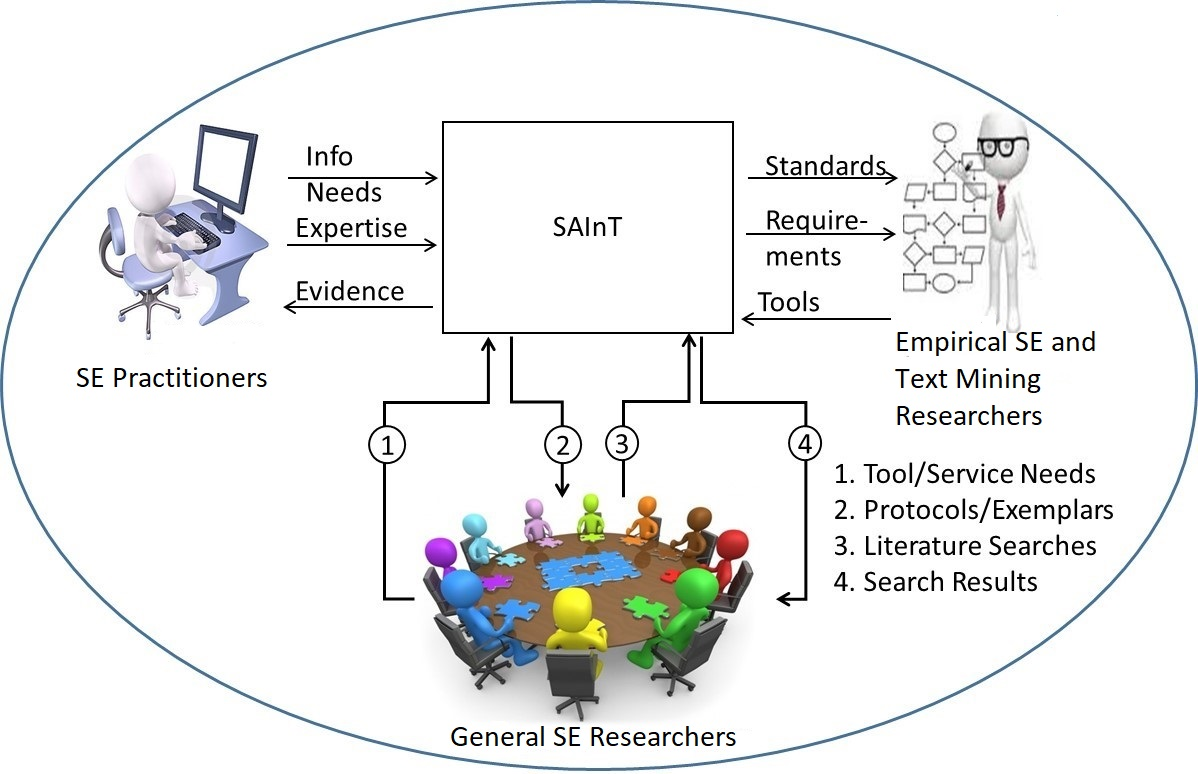
\includegraphics[width=4.5in]{ResearchEnabled}
	\caption{Communities Serviced by {\IT}.}
	\label{figure-ResearchEnabled}
\end{figure}
\item {\em Community \#1: General Software Engineering Researchers}
 

 One reason to augment standard SLRs with AI tools (as done in {\IT}) is that the SE field urgently  needs to rethink its core premises using more of the current evidence.
We say this since currently there is much
disagreement on what many factors most effect software projects.
For example, according to Passos et al.,  developers often assume that the lessons they learn from a few past projects are general to all their future projects. 
They comment, ``past experiences were taken into account without much consideration for their context''~\cite{Pa11}. 
 J{\o}rgensen \& Gruschke offer a similar warning. 
They report that the supposed software engineering ``gurus'' rarely use lessons from past projects to improve their future reasoning and that such poor past advice can be detrimental to new projects~\cite{Jo09}.
 Other studies have shown some widely-held views are now questionable given new evidence.
	Devanbu et al. examined responses from 564 Microsoft software developers from around
	the world. 
	They comment programmer beliefs can vary with each project, but do not necessarily correspond with actual evidence in that project~\cite{De16}. 

The Le~Goues, Shaw et al.~\cite{Goues18} paper  characterizes such uncertainties
as symptoms of a researcher
  community that is poorly defining its research outputs. They say:
  \begin{quote}
  {\em When engineers seek answers to their practical problems, ``perfect'' scientific knowledge is not always available. If it's not, engineers readily accept ``good-enough'' evidence: case studies, small-scale experiments, blog posts, or even advice from acknowledged experts.}~\cite{Goues18} 
  \end{quote}
Their challenge to the community is to provide better ``good-enough'' evidence. In this proposal,
we explore the application of AI tools to text mining to provide such good enough evidence via AI-augmented literature reviews.
\item
{\em Community \#2:  Empirical Software Engineering and Text Mining Researchers}
We also plan to support these researchers by providing a platform to experiment  with  different techniques  and  workflows. Empirical software engineering researchers have established some recommended workflows (e.g. pilot search and keyword refinement~\cite{keele2007guidelines}) and strategies (e.g. snowballing~\cite{jalali2012systematic}) to improve the efficiency and quality of SLRs. Meanwhile, many text mining researchers have selected SLRs as case studies to test the effectiveness of different machine learning algorithms (e.g. active learning~\cite{Yu2018} and visual text mining~\cite{Felizardo2010An}). {\IT} as a platform will facilitate the testing of mix-and-matching different workflows, strategies, and algorithms, thus benefit the research of both empirical software engineering and text mining. In addition, {\IT} will be beneficial as a testbed for latest developed algorithms from text mining and machine learning, e.g. word2vec, deep neural networks, named entity recognition, part-of-speech tagging, etc.

\item {\em Community \#3: Software Engineering Practitioners}
In addition to the benefits to researchers described above, the numerous consumers that utilize the results of SLRs will also benefit from the work.  
Practitioners and executives in industry utilize SLR results to identify best practices and to guide decision making.  
Industrial software engineers will benefit from more applied and relevant research that they can commission.
Other researchers have already begun building methods (e.g. Visual Abstracts~\cite{VisualAbstracts}) for representing the findings of SLRs in a format that is useful to practitioners.
By helping researchers produce more SLRs that represent all of the literature, {\IT} will help the results presented to industry be more complete and accurate.
\ee
\ei
\vspace{8pt}